\documentclass[a4paper,12pt]{article}

% Layout
\usepackage[a4paper, left=2cm, right=2cm, top=1.5cm, bottom=3cm]{geometry} % kleinere Ränder
\usepackage{parskip}

% Umlaute in der Datei erlauben, auf Deutsch umstellen
\usepackage{fontspec}
\usepackage{lmodern}
\usepackage[english, ngerman]{babel}

% Mathesymbole und Ähnliches
\usepackage{amsmath}
\usepackage{amsthm}
\usepackage{mathtools}
\usepackage{amssymb}
\usepackage{microtype}
\usepackage{stmaryrd}
\usepackage{MnSymbol}
\usepackage{bussproofs}		% Sequenzenkalkül
\usepackage{xcolor}

% Grafiken und PDFs einfügen
\usepackage{graphicx}
\usepackage{pdfpages}
\usepackage{float}

% PDF-Tools
\usepackage[hidelinks, unicode]{hyperref}

% Abbildungen
\usepackage{tikz}
\usetikzlibrary{arrows,calc,positioning}
\tikzset{ 
   state/.style={circle,fill,inner sep=2pt,label=below:#1\strut},
   arrow/.style={->, shorten <=3pt, shorten >=3pt, >=stealth',thick},
   knoten/.style={draw, circle, minimum size=8mm}} 
   
% Infoboxen 
\definecolor{orange}{RGB}{230,159,0}
\definecolor{darkgray}{RGB}{70,90,70}

\usepackage{tcolorbox}

\newenvironment{LP}[1]{%
\begin{minipage}{0.48\textwidth}
\begin{tcolorbox}[colback=orange!20!white, colframe=orange!80!black, title={\sffamily \textbf{#1}}]
}{
\end{tcolorbox}
\end{minipage}}

\newenvironment{alg}[1]{%
\begin{tcolorbox}[colback=red!15!white, colframe=red!85!black, title={\sffamily \textbf{#1}}]
}{
\end{tcolorbox}}

\newenvironment{info}[1]{%
\begin{tcolorbox}[colback=darkgray!15!white, colframe=darkgray!75!black, title={\sffamily \textbf{#1}}]
}{
\end{tcolorbox}}


% Reelle, Natürliche, Ganze, Rationale Zahlen
\newcommand{\R}{\ensuremath{\mathbb{R}}}
\newcommand{\N}{\ensuremath{\mathbb{N}}}
\newcommand{\Z}{\ensuremath{\mathbb{Z}}}
\newcommand{\Q}{\ensuremath{\mathbb{Q}}}

% Fraktur für Strukturen
\newcommand{\A}{\ensuremath{\mathfrak A}}
\newcommand{\B}{\ensuremath{\mathfrak B}}
\newcommand{\I}{\ensuremath{\mathfrak I}}

% Körper
\newcommand{\K}{\ensuremath{\mathcal{K}}}
%\newcommand{\G}{\ensuremath{\mathcal{G}}}

% Makros für logische Operatoren
\newcommand{\xor}{\ensuremath{\oplus}} % exklusives oder
\newcommand{\impl}{\ensuremath{\rightarrow}} % logische Implikation
\newcommand{\Lor}{\ensuremath{\bigvee}}
\newcommand{\Land}{\ensuremath{\bigwedge}}

% Meistens ist \varphi schöner als \phi, genauso bei \theta
\renewcommand{\phi}{\varphi}
\renewcommand{\theta}{\vartheta}
\renewcommand{\setminus}{\backslash}

\newcommand*{\todo}{\textbf{\textcolor{red}{TODO}}}		% big, red, apparent TODO

% SEQUENZENKALKÜL
\usepackage{bussproofs}
\newcommand{\yields}{\ensuremath{\mathrel{\Rightarrow}}}

% Aufzählungen anpassen (alternativ: \arabic, \alph)
\renewcommand{\labelenumi}{(\roman{enumi})}

% BITTE NICHT ÄNDERN: interne Kommandos für die Informationen (Blattnummer, Gruppe, ...)
\newcounter{sheet}
\newcommand{\printsheet}{\arabic{sheet}}


\newcommand{\printgroup}{?}
\newcommand{\group}[1]{%
\renewcommand{\printgroup}{#1}%
}

\newcommand{\printmembers}{}
\newcommand{\printmember}[3]{{#2} {#3} & {#1} \\}

\newtheorem{proposition}{Proposition}[sheet]

% Für Vektoren
\newcommand{\myvec}[1]{\ensuremath{\begin{pmatrix}#1\end{pmatrix}}}
\def\spvec#1{\left(\vcenter{\halign{\hfil$##$\hfil\cr \spvecA#1;;}}\right)}
\def\spvecA#1;{\if;#1;\else #1\cr \expandafter \spvecA \fi}

\newcommand{\pdfmembers}{}
\newcommand{\pdfmember}[3]{{#1} {#3}, {#2}; }

\newcommand{\member}[3]{%
\expandafter\renewcommand\expandafter\printmembers\expandafter{\printmembers\printmember{#1}{#2}{#3}}%
\expandafter\renewcommand\expandafter\pdfmembers\expandafter{\pdfmembers\pdfmember{#1}{#2}{#3}}%
}

\AtBeginDocument{\hypersetup{
    pdftitle = {Übungsblatt \printsheet},
    pdfauthor = {Abgabegruppe \printgroup: \pdfmembers},
    pdfsubject = {Concurrency Theory}
}}

% <-------- HIER alle Informationen eintragen ========================
\setcounter{sheet}{2} % Nummer des Blatts

% alle Gruppenmitglieder in der Form \member{Matrikelnummer}{Vorname}{Nachname}
\member{5481114}{Danje}{Petersen}
\member{5174511}{Marc}{Majohr}

\begin{document}

% Kopfzeile
{\raggedright
\begin{tabular}{l}
    Concurrency Theory \\
    SS 2024 \\
\end{tabular}}
\hfill
{\Large Übung 0\printsheet}
\hfill
\begin{tabular}{l l}
\printmembers
\end{tabular}
\hrule


% <-------- HIER beginnt die Lösung ========================

\section*{Aufgabe \printsheet.1}
\begin{proposition} For a directed graph $G=(V;E)$ and a cycle $c$ in G, $\psi(c)$ is a solution of the Kirchhoff equation for $G$, i.e.:
\[\forall v \in V: \sum_{e=(-,v)} \psi(e) - \sum_{e=(v,-)} \psi(e) = 0\] \end{proposition}
\begin{proof}
Per Induktion über Anzahl primitiver Zykel in $c$. \\
\textbf{Induktionsanfang:} Sei $|c| = 0$ oder ein primitiver Zykel. \\
Für $|c| = 0$ gilt $\forall v \in V: \sum_{e=(v,-)} \psi(e) = \sum_{e=(-,v)} \psi(e) = 0$ und dadurch auch 
\[\forall v \in V: \sum_{e=(-,v)} \psi(e) - \sum_{e=(v,-)} \psi(e) = 0\]
Für $c =$ primitiver Zykel gilt, dass jeder Knoten höchstens einmal besucht wird. Dafür wird eine eingehende und eine ausgehende Kante benötigt. Somit gilt für jeden Knoten in $c$:
\[\forall v \in c: \sum_{e=(-,v)} \psi(e) = \sum_{e=(v,-)} \psi(e) = 1\]
und somit:
\[\forall v \in V: \sum_{e=(-,v)} \psi(e) - \sum_{e=(v,-)} \psi(e) = 1-1 = 0\]

\textbf{Induktionsschritt:} Sei $c$ ein Zykel, der sich in $n+1$ primitive Zykel $c_1,...,c_n,c_{n+1}$ aufteilen lässt. \\
Somit gilt:
\begin{align*}
&\forall v \in V: \sum_{e=(-,v)} \psi(e) - \sum_{e=(v,-)} \psi(e) = 0\\
&\Leftrightarrow \forall v \in c: \sum_{e=(-,v)} \psi(e) - \sum_{e=(v,-)} \psi(e) = 0 \\
&\Leftrightarrow \forall c_i \in \{c_1,\dots c_{n+1}\}: \forall v \in c_i: \sum_{e=(-,v)} \psi(e) - \sum_{e=(v,-)} \psi(e) = 0\\
&\overset{IV}{\Leftrightarrow} \forall v \in c_{n+1}: \sum_{e=(-,v)} \psi(e) - \sum_{e=(v,-)} \psi(e) = 0\\
&\Leftrightarrow 1 - 1 =  0
\end{align*}
\end{proof}

\section*{Aufgabe \printsheet.2}
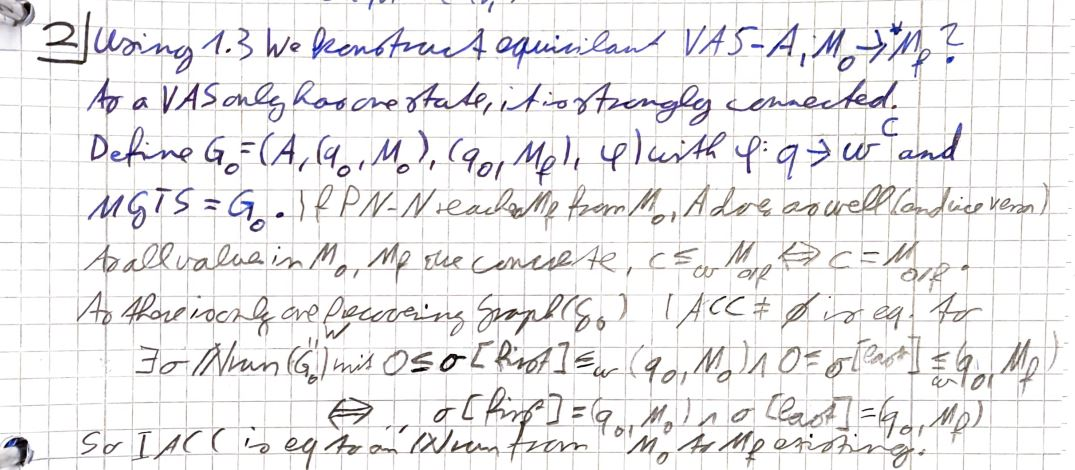
\includegraphics[scale=0.65]{2}


\section*{Aufgabe \printsheet.3}
\subsection*{(a)}
\begin{align*}
Char(W) &=& Char(G_0) \land Char(G_1) \land MARK(G_0.t_7.G_1) \\
&=& \forall t_i \in W.T x[t_i] \geq 0 \land MARK(G_0) \land KIRCH(G_0) \land IACC(G_0) \\ 
&\land&  MARK(G_1) \land KIRCH(G_1) \land IACC(G_1) \land MARK(G_0.t_7.G_1)
\end{align*}
Kirchhoffgleichung von $G_0$ ist immer wahr, da $x[t_0] - x[t_0] = 0$.
\begin{align*}
MARK(G_0) &= x[G_0,in,1] - x[G_0,out,1] = 0 \\ 
&\land x[G_0,in,2] - x[G_0,out,2] = 0 \\
& \land x[G_0,in,3] + 2x[t_0] - x[G_0,out,3] = 0
\end{align*}
\begin{align*}
IACC(G_0) &= 0 \leq_\omega x[G_0,in] \leq_\omega \myvec{0&0&0} \\
&\land 0 \leq_\omega x[G_0,out] \leq_\omega \myvec{0&0&\omega}
\end{align*}
\begin{align*}
MARK(G_1) &= x[G_1,in,1] - x[t_2] - x[t_3] + x[t_4] + 2 x[t_5] - x[G_1,out,1] = 0 \\ 
&\land x[G_1,in,2] + 2x[t_1] + 2x[t_4] - 7x[t_5] - x[t_6] - x[G_1,out,2] = 0 \\
& \land x[G_1,in,3] - 6x[t_4] - x[G_1,out,3] = 0
\end{align*}
\begin{align*}
KIRCH(G_1) &= x[t_6] + x[t_3] - x[t_5] - x[t_4] - x[t_6] = 0 \\
&\land x[t_2] + x[t_4] - x[t_3] = 0 \\
&\land x[t_5] + x[t_1] - x[t_1] - x[t_2] = 0
\end{align*}
\begin{align*}
IACC(G_0) &= 0 \leq_\omega x[G_1,in] \leq_\omega \myvec{0&0&\omega} \\
&\land 0 \leq_\omega x[G_1,out] \leq_\omega \myvec{0&1&0}
\end{align*}
\begin{align*}
MARK(G_0.t_7.G_1) &= x[G_0,in,1] - x[G_1,out,1] = 0 \\ 
&\land x[G_0,in,2] - x[G_1,out,2] = 0 \\
& \land x[G_0,in,3] - 2x[t_7] - x[G_1,out,3] = 0
\end{align*}

\subsection*{(b)}
$G_0:$ \\
Up-pumping sequence $\sigma_1 = t_0$

Down-pumping sequence $\sigma_2 = \varepsilon$

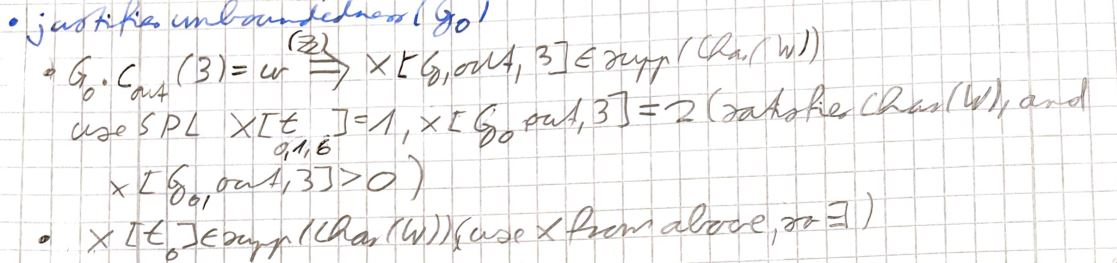
\includegraphics[scale=0.6]{3b0.jpg}


$G_1:$ \\
Up-pumping sequence $\sigma_3 = t_4.t_3$

Down-pumping sequence $\sigma_4 = t_6$

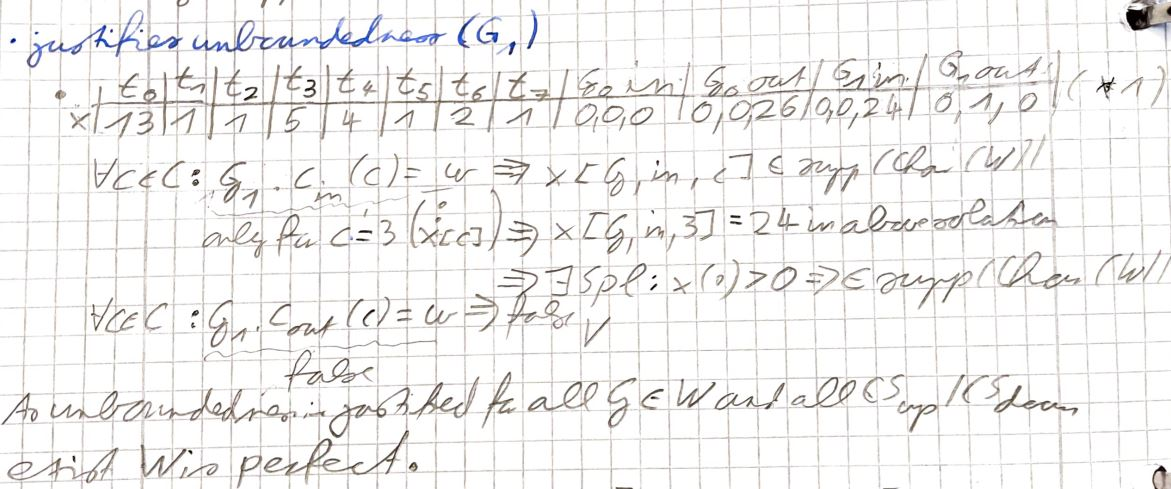
\includegraphics[scale=0.57]{3b1}

\subsection*{(c)}
\[s_h = (t_0)^4.t_4.t_3.t_5.(t_1)^3.t_2.t_3.t_6\]

\subsection*{(d)}


\subsection*{(e)}



\section*{Aufgabe \printsheet.4}
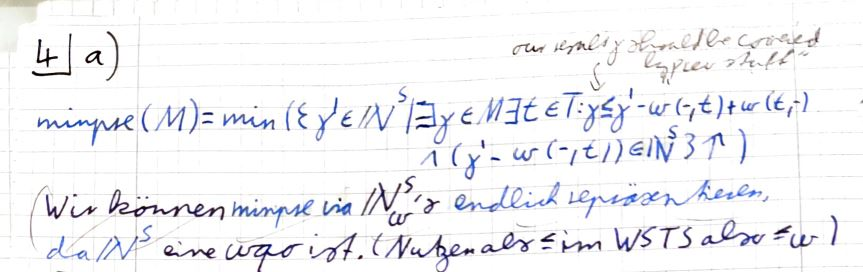
\includegraphics[scale=0.6]{4a}
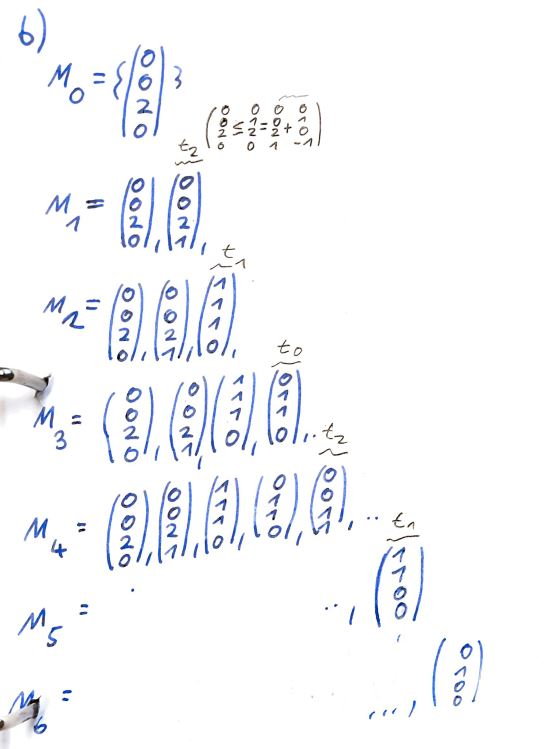
\includegraphics[scale=0.6]{4b}



\end{document}
